\documentclass[a4paper]{article}
\usepackage[utf8]{inputenc}
\usepackage{fancyhdr}
\usepackage{vmargin}
\usepackage{listings}

%nicer tables
\usepackage{booktabs}

\usepackage{graphicx}

\usepackage{float}

\usepackage{color}
\usepackage{url}
\usepackage{hyperref}

\usepackage{enumerate}

\usepackage[backend=biber]{biblatex}

\usepackage{multicol}
\setlength{\columnsep}{1cm}
\setlength{\headheight}{36pt}

\definecolor{bluekeywords}{rgb}{0.13,0.13,1}
\definecolor{greencomments}{rgb}{0,0.5,0}
\definecolor{redstrings}{rgb}{0.9,0,0}



%
\usepackage{amsmath, amsthm, amssymb}
\usepackage[ngerman, english]{babel}
\usepackage{marvosym}
\usepackage{graphics}
\usepackage{extarrows}
\usepackage{forloop}
\usepackage{mathtools}

\usepackage[]{algorithm2e}

\usepackage{hyperref}% http://ctan.org/pkg/hyperref
\usepackage{cleveref}% http://ctan.org/pkg/cleveref
\usepackage{lipsum}% http://ctan.org/pkg/lipsum
\newtheorem{definition}{Definition}
\newtheorem{theorem}{Theorem}
\newtheorem{lemma}{Lemma}
\newtheorem{preliminary}{Preliminary}
\newtheorem{notation}{Notation}
\newtheorem{property}{Property}
\newtheorem{corollary}{Corollary}
\newtheorem{example}{Example}
\newtheorem{hypothesis}{Hypothesis}

\crefname{theorem}{Theorem}{Theorems}
\crefname{definition}{Definition}{Definitions}
\crefname{lemma}{Lemma}{Lemmas}
\crefname{preliminary}{Preliminary}{Preliminaries}
\crefname{notation}{Notation}{Notations}
\crefname{property}{Property}{Properties}
\crefname{corollary}{Corollary}{Corollaries}
\crefname{example}{Example}{Examples}
\crefname{hypothesis}{Hypothesis}{Hypotheses}

\newenvironment{beweis}{\begin{proof}[Beweis]}{\end{proof}}
%



\lstset{language=Python,
showspaces=false,
showtabs=false,
breaklines=true,
showstringspaces=false,
breakatwhitespace=true,
escapeinside={(*@}{@*)},
commentstyle=\color{greencomments},
keywordstyle=\color{bluekeywords}\bfseries,
stringstyle=\color{redstrings},
basicstyle=\ttfamily
}


\setlength{\parindent}{0pt}
\setlength{\parskip}{5pt}

\frenchspacing
\pagestyle{fancy}
\sloppy 

\markright{headline}

\addbibresource{references.bib}

\begin{document}

\lhead{\begin{tabular}{l}
\\
Neural Networks\\
WiSe 2020/2021\\
\end{tabular}}

\rhead{\begin{tabular}{r}
Assignment 6\\
Simon Laurent Lebailly, 2549365, s9sileba@teams.uni-saarland.de\\%% <=== Also HERE if you have a team mateUpdate Name HERE !!! 
Christian Mathieu Schmidt, 2537621, s9cmscmi@teams.uni-saarland.de
\end{tabular}}




\section*{Exercise 7.1: $L_1$ and $L_2$ Regularization}
    \subsection*{a)}
        \begin{center}
            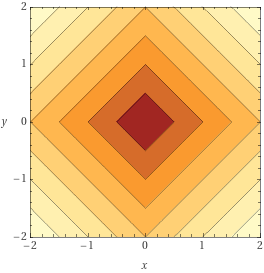
\includegraphics[width=55mm]{Assignment 7/L1(2).png}
            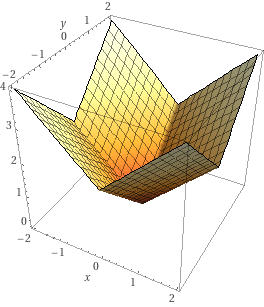
\includegraphics[width=55mm]{Assignment 7/L1(1).png}\\
            \caption{$L_1$ Contour-plot and 3D-plot (plotted at https://www.wolframalpha.com)}
        \end{center}
        \begin{center}
            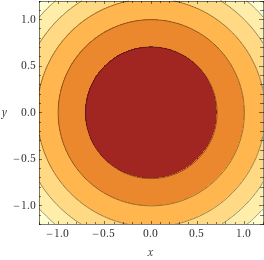
\includegraphics[width=55mm]{Assignment 7/L2(2).png}
            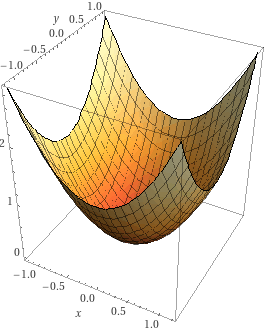
\includegraphics[width=55mm]{Assignment 7/L2(1).png}\\
            \caption{$L_2$ Contour-plot and 3D-plot (plotted at https://www.wolframalpha.com)}
        \end{center}


    \subsection*{b)}
        $L_1$ produces a spase model, because most of its parameters will become equal to zero, provided the hyperparameter is large enough.
        So $L_1$ performs feature selection by deciding which features are essential for prediction and which are not.
        So $L_1$ is prefered, if we want to increase the model explainability.

    
    \subsection*{c)}
        Yes it is possible and is called "elastic net regularization", which has $L_1$ and $L_2$ regularizations as special cases.
        Elastic net regularization linearly combines the L1 and L2 penalties of the lasso and ridge methods and can be reduced to the linear support vector machine.\footnote{https://www.aaai.org/ocs/index.php/AAAI/AAAI15/paper/view/9856}
        The reduction immediately enables the use of highly optimized SVM solvers for elastic net problems. It also enables the use of GPU acceleration, which is often already used for large-scale SVM solvers.\footnote{https://ttic.uchicago.edu/~cotter/projects/gtsvm/}
    
    \subsection*{d)}
        Regularization encompasses methods that force the learning algorithm to build a less complex model.
        In practice, that often leads to slightly higher bias but reduces the variance significantly (bias-variance tradeoff).
        The idea of regularization is to modify the objective function by adding a penalizing term whose value is higher when the model is more complex.
        So, regularization decreases the generalization error by increasing, or in better words not reducing, the training error.
        This is only important if there is a risk to overfit the model. 

    
    \subsection*{e)}
    

    
    \subsection*{f)}
    

    


\newpage
\section*{Exercise 7.2: Multi-Task Learning and Data Augmentation}
    \subsection*{a)}
    
    \subsection*{b)}



\newpage
\section*{Exercise 7.3: Early Stopping}
    \subsection*{a)}
        Under the assumption (i) $|1-\epsilon\lambda_j| < 1$, it holds that
        \begin{align}
            \lim_{\tau \rightarrow \infty} \omega^{\tau}_j &= \lim_{\tau \rightarrow \infty} \{1 - (\underbrace{1 - \epsilon\lambda_j}_{< 1\ (i)})^{\tau}\} \omega^{*}_j\\
            &= \{1 - 0\} \omega^{*}_j = \omega^{*}_j
        \end{align}
        $\Rightarrow$ If the number of steps $\tau$ goes to infinity, then each component of the weight vector $\omega^{\tau}_j$ converges to the corresponding component $\omega^*_j$ of the minimum! Thus it is valid for the weight vector $\omega$ that 
        \begin{align}
            \lim_{\tau \rightarrow \infty} \omega^{\tau} &= \omega^*
        \end{align}
    
    \subsection*{b)}
    
    \subsection*{c)}



\newpage
\section*{Exercise 7.4: Universal Approximation Theorem}
    \subsection*{a)}
    
    \subsection*{b)}
    
    \subsection*{c)}






\end{document}
